\section{Partie 1 : Plateforme}
    \subsection{Plateforme : Généralités}
        \begin{frame}[allowframebreaks]{Plateforme}
            \begin{columns}
                \begin{column}{0.5\textwidth}
                    \begin{exampleblock}{}
                        \begin{itemize}
                            \item Schneider Electric
                            \item Composé de 2 automates : M340 et M580
                            \item Nombreux capteurs disponibles
                        \end{itemize}
                    \end{exampleblock}
                \end{column}\hfill
                \begin{column}{0.5\textwidth}
                    \begin{figure}
                        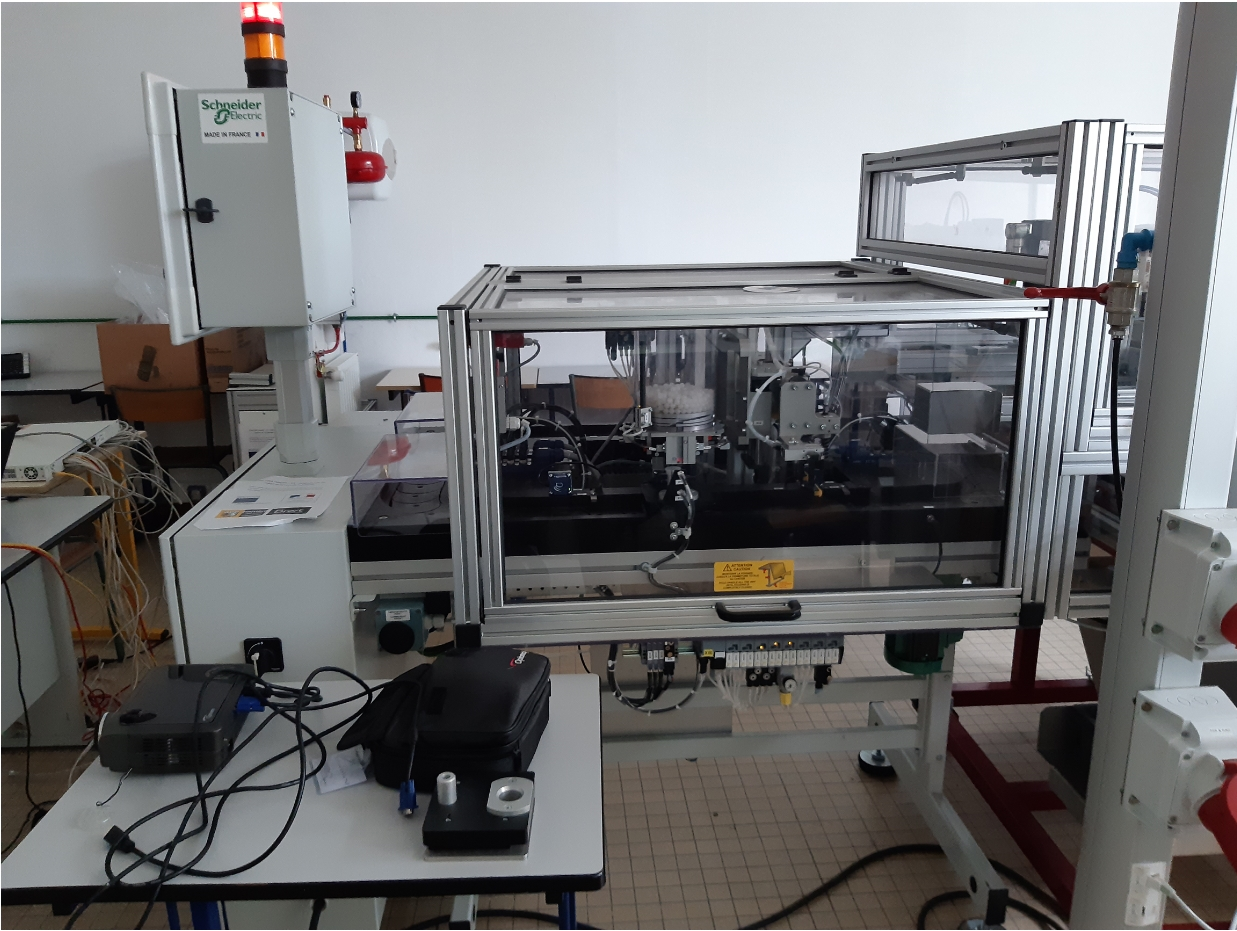
\includegraphics[width=1\linewidth]{images/plateforme.jpg}
                        \caption*{Plateforme industrielle}
                    \end{figure}
                \end{column}
            \end{columns}
        \end{frame}
%
% ---------------------------------------------------------------- %
    \subsection{Plateforme : Travail effectué}
        \begin{frame}[allowframebreaks]
             \begin{block}{}
                \begin{itemize}
                    \setbeamertemplate{itemize item}[square]
                    \item Lecture manuelle des données sur le logiciel \textit{Unity Pro XLS}
                    \item Création d'un programme Java :
                    \begin{itemize}
                        \item Lecture des registres de l'automate (exemples : \%M103 \& \%MW150)
                        \item Enregistrement dans une base de données MS SQL Server 2014
                    \end{itemize}
                \end{itemize}
            \end{block}
            
            \begin{columns}[T]
                \begin{column}{0.5\textwidth}
                    \begin{figure}[H]
                        \centering
                        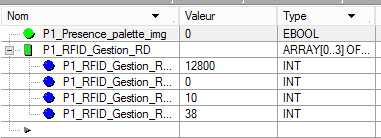
\includegraphics[width=1\linewidth]{images/regUnity.png}
                        \caption*{Exemple sur \textit{Unity Pro XLS}}
                    \end{figure}
                \end{column}\hfill
                \begin{column}{0.5\textwidth}
                    \begin{figure}[H]
                        \centering
                        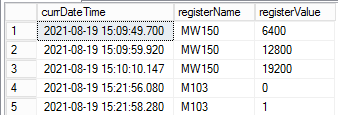
\includegraphics[width=1\linewidth]{images/exempleSQLSave.png}
                        \caption*{Contenu de la base de données}
                    \end{figure}
                \end{column}
            \end{columns}
        \end{frame}
%
% ---------------------------------------------------------------- %
    \subsection{Plateforme : Architecture}
        \begin{frame}[allowframebreaks]
            \begin{figure}
                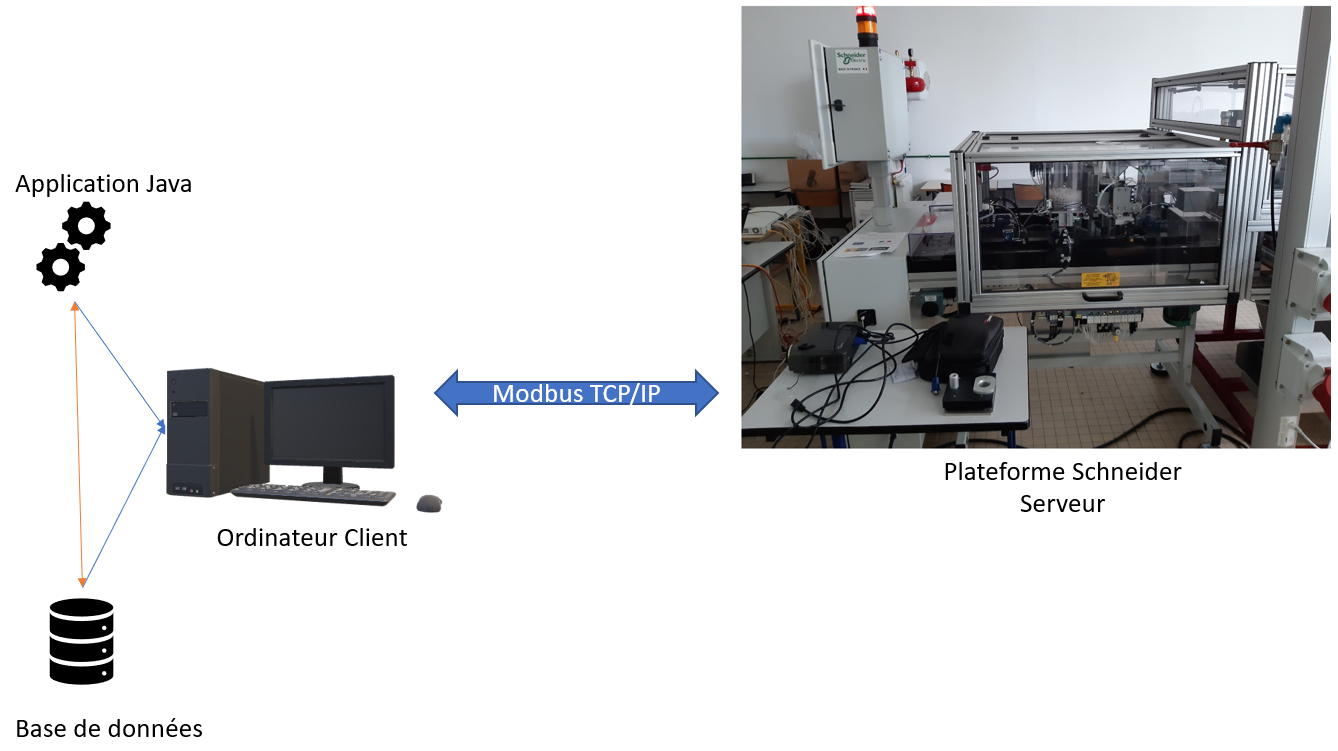
\includegraphics[width=1\linewidth]{images/architectureGeneraleNoDrone.png}
            \end{figure}
        \end{frame}
%
% ---------------------------------------------------------------- %